% !TEX root=./report.tex

\subsection{Static calibration}
In the following we evaluate the implemented static calibration algorithm and assess the possible algorithmic and systematic errors.

%%%%%%%%%%%%%%%%%%%%%%%%%%%%%%%%%%%%%%%%%%%%%%%%%%%%%%%%%%%%%%%%%%%%%%%%%%%%%%%%%%%%%%%%%%%%%%%%%%%%%%%%%%%%%%%%%%%%
%%%%%%%%%%%%%%%%%%%%%%%%%%%%%%%%%%%%%%%%%%%%%%%%%%%%%%%%%%%%%%%%%%%%%%%%%%%%%%%%%%%%%%%%%%%%%%%%%%%%%%%%%%%%%%%%%%%%
%%%%%%%%%%%%%%%%%%%%%%%%%%%%%%%%%%%%%%%%%%%%%%%%%%%%%%%%%%%%%%%%%%%%%%%%%%%%%%%%%%%%%%%%%%%%%%%%%%%%%%%%%%%%%%%%%%%%

\subsubsection{Ensure no Systematic Error}

\begin{figure*}[t]
    \centering
    \begin{tabular}{cc}
      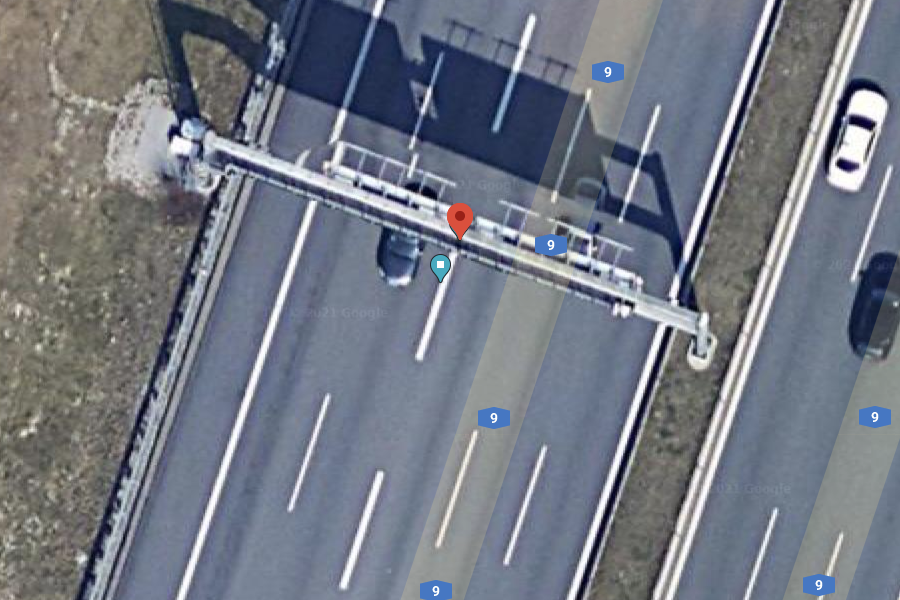
\includegraphics[width=0.45 \linewidth]{images/calibration/google_maps_s40_n.png} &
      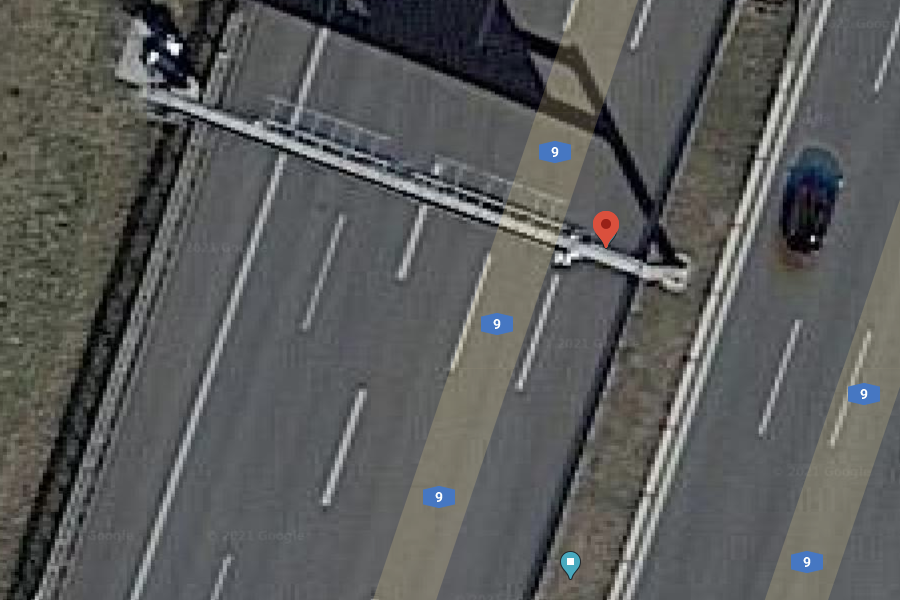
\includegraphics[width=0.45 \linewidth]{images/calibration/google_maps_s50_s.png} 
  \end{tabular}
  \caption{Left: The positions of the cameras \camsn{4} (red) and \camsf{4} (blue) and their respective looking directions (green). 
  Right: The positions of the cameras \camsn{5} (red) and \camsf{5} (blue) and their respective looking directions (green). 
  The rotations of the cameras are in a reasonable range so that the cameras look along the highway as expected. 
  All cameras, except the \camsf{5} camera, are within reasonable translational bounds around their real world location as \autoref{sec:static_calibration_expectable_error} shows.
  }
  \label{fig:static_calibration_google_maps}
  \end{figure*}

We solve the BA problem proposed in \autoref{sec:static_calibration_approach} by minimizing the reprojection-error as formulated in \autoref{eq:static_calibration_rerpojection_error}.
The algorithm converges to a pair of optimal translation $T$ and rotation $R$ values for the camera pose.
These $T, R$ values best describe the camera pose relative to the mapped objects as stated in \autoref{eq:static_calibration_reprojection}.

Using a maps provider we assured that the resulting values are within reasonable ranges and that there are no systematic errors in the optimization.
\autoref{fig:static_calibration_google_maps} displays the positions of the four cameras and their respective looking directions. 
It shows that except for the \camsf{5} the expected position is within the expectable range around the actual position.
All cameras are looking along the highway as expected. 

%%%%%%%%%%%%%%%%%%%%%%%%%%%%%%%%%%%%%%%%%%%%%%%%%%%%%%%%%%%%%%%%%%%%%%%%%%%%%%%%%%%%%%%%%%%%%%%%%%%%%%%%%%%%%%%%%%%%
%%%%%%%%%%%%%%%%%%%%%%%%%%%%%%%%%%%%%%%%%%%%%%%%%%%%%%%%%%%%%%%%%%%%%%%%%%%%%%%%%%%%%%%%%%%%%%%%%%%%%%%%%%%%%%%%%%%%
%%%%%%%%%%%%%%%%%%%%%%%%%%%%%%%%%%%%%%%%%%%%%%%%%%%%%%%%%%%%%%%%%%%%%%%%%%%%%%%%%%%%%%%%%%%%%%%%%%%%%%%%%%%%%%%%%%%%

\subsubsection{Number of Correspondences Needed for Convergence}
\label{sec:static_calibration_number_points}
The correspondences build up a system of linear equations as described in \autoref{eq:static_calibration_reprojection}.
This system of equations is solvable if the number of constraints on the parameters is equal to or exceeds the degrees of freedom in the system, thus being over constrained.
This is the case if for the number $\left\lvert C \right\rvert$ of correspondences it holds that
\begin{equation}
  \begin{split}
  2 * \left\lvert C \right\rvert \quad \geq& \quad 5 + 3 + 3 + 1 * \left\lvert C \right\rvert \\
  \left\lvert C \right\rvert \quad \geq& \quad 11 
\end{split}
\end{equation} 

as each of the expected pixels $\hat{p}_c$ gives us two constraints and we optimize for the 5 intrinsic parameters, 3 extrinsic translation parameters, 3 extrinsic rotation parameters and one $\lambda_c$ parameter per correspondence.
It shows that 11 points are enough to recover the pose, though more points improve the robustness of the algorithm.

%%%%%%%%%%%%%%%%%%%%%%%%%%%%%%%%%%%%%%%%%%%%%%%%%%%%%%%%%%%%%%%%%%%%%%%%%%%%%%%%%%%%%%%%%%%%%%%%%%%%%%%%%%%%%%%%%%%%
%%%%%%%%%%%%%%%%%%%%%%%%%%%%%%%%%%%%%%%%%%%%%%%%%%%%%%%%%%%%%%%%%%%%%%%%%%%%%%%%%%%%%%%%%%%%%%%%%%%%%%%%%%%%%%%%%%%%
%%%%%%%%%%%%%%%%%%%%%%%%%%%%%%%%%%%%%%%%%%%%%%%%%%%%%%%%%%%%%%%%%%%%%%%%%%%%%%%%%%%%%%%%%%%%%%%%%%%%%%%%%%%%%%%%%%%%

\subsubsection{Structure of Correspondences}
We empirically see that recovering the camera pose performs best when there are at least two correspondences per object.
These correspondences need to be the top and bottom most visible pixel of the object.
If there exists only 1 or a low number of dense packed pixels the algorithm cannot precisely recover the camera pose as it is free to move the correspondences along the center line of the object.
The algorithm therefore cannot distinguish solutions where it places the camera low, thus projecting a high point of an object to a low pixel correspondence, and solutions where it places the camera high and lowers the world position of the correspondence along the center line.

% We thus conclude that the best solution is recovered the more the pixels fill the whole object, and the more spread to the top and bottom of the object the correspondences are. 


%%%%%%%%%%%%%%%%%%%%%%%%%%%%%%%%%%%%%%%%%%%%%%%%%%%%%%%%%%%%%%%%%%%%%%%%%%%%%%%%%%%%%%%%%%%%%%%%%%%%%%%%%%%%%%%%%%%%
%%%%%%%%%%%%%%%%%%%%%%%%%%%%%%%%%%%%%%%%%%%%%%%%%%%%%%%%%%%%%%%%%%%%%%%%%%%%%%%%%%%%%%%%%%%%%%%%%%%%%%%%%%%%%%%%%%%%
%%%%%%%%%%%%%%%%%%%%%%%%%%%%%%%%%%%%%%%%%%%%%%%%%%%%%%%%%%%%%%%%%%%%%%%%%%%%%%%%%%%%%%%%%%%%%%%%%%%%%%%%%%%%%%%%%%%%

\subsubsection{Expectable Error Bounds}
\label{sec:static_calibration_expectable_error}

Due to measurement uncertainty in the camera sensors we expect some remaining error after pose estimation.
We derive a lower bound on this error starting from the optimized focal length $f_px$ in pixels, the sensor width $w_{mm}$ in millimeters and $w_{px}$ in pixels.
We use the focal length in millimeters given by 
\begin{equation}
  f_{mm} = f_{px} * \frac{w_{mm}}{w_{px}}
\end{equation}
to calculate the field of view (FOV) in radians by 
\begin{equation}
  FOV_x = 2 * \arctan \left(\frac{f_{mm}}{2 * w_{mm}}\right)
\end{equation} 
Equivalent the $FOV_y$ with the height of the sensor $h_{mm}$.
The angle spanned by each pixel is calculated by
\begin{equation}
  \alpha_{px} = \frac{w_{px}}{FOV_x}
\end{equation} 

Using the pythagorean formula we can then calculate the uncertainty 
\begin{equation}
  u = \tan (\alpha_{px}) * d
\end{equation}
of the camera as the spanned meters per pixel relative to the distance $d$ from the camera.

\begin{table}
  \begin{center}
    \begin{tabular}{ |c | c | c| c| c| c |}
      \hline
      Camera & $f_{px}$ & $FOV_x [^{\circ}]$ & $\alpha_{px}[rad]$ & $d [m]$ & $u [cm]$ \\
      \hline
      \camsf{4} & 8591 & 12.753 & $1.16e^{-4}$ & 200 & 2.32 \\
      \camsf{4} & 8591 & 12.753 & $1.16e^{-4}$ & 650 & 7.54 \\
      \hline
      \camsn{4} & 2735 & 38.678 & $3.52e^{-4}$ & 25 & 0.88 \\
      \camsn{4} & 2735 & 38.678 & $3.52e^{-4}$ & 450 & 15.82 \\
      \hline
      \camsf{5} & 8868 & 12.357 & $1.12e^{-4}$ & 200 & 2.22 \\
      \camsf{5} & 8868 & 12.357 & $1.12e^{-4}$ & 650 & 7.30 \\
      \hline
      \camsn{5} & 2747 & 38.527 & $3.50e^{-4}$ & 25 & 0.88\\
      \camsn{5} & 2747 & 38.527 & $3.50e^{-4}$ & 450 & 15.76 \\
      \hline
    \end{tabular}
  \end{center}
  \caption{
    The focal lengths $f_{px}$, fields of view $FOV_x [^{\circ}]$ and spanned angle per pixel $\alpha_{px}[rad]$ compared to the measurement uncertainty $u [cm]$ at some distance $d [m]$ from the cameras.
    It shows a linear increase of the uncertainty proportional to the distance of the object from the camera.  
  }
  \label{tab:static_calibration_camera_uncertainty}
\end{table}

\autoref{tab:static_calibration_camera_uncertainty} displays the uncertainty for our cameras.
It shows that the far cameras cannot distinguish between points that are $\sim 2.2 cm$ at the nearest visible distance from the camera ranging up to $\sim 7.54 cm$ at the farthest distance.
The near cameras cannot distinguish between points that are $\sim 0.88 cm$ at the nearest visible distance from the camera ranging up to $\sim 15.82 cm$ at the farthest distance.

The highest possible achievable precision for the translational parameters of the camera is bound by the uncertainty in the measurements, as a misplacement of the camera can only be detected if it is higher than the sensor uncertainty.
Nonetheless, in practice the imprecision will sum up and the translation parameters will drift inevitable. 
This implies that objects in close distance to the camera are more reliable when estimating the translation.

The rotational parameters can be estimated more precisely, as small rotational deviations introduce large deviations in the objects projected pixels.
The expectable precision for the rotation is thus bound by the angle $a_{px}$ spanned per pixel, as a deviation by one $a_{px}$ would project the objects onto the next pixel.
This implies that the precision of the rotation is at least in the range of $1.12 * 10^{-4}$ to $3.52 * 10^{-4}$ radians. 

%%%%%%%%%%%%%%%%%%%%%%%%%%%%%%%%%%%%%%%%%%%%%%%%%%%%%%%%%%%%%%%%%%%%%%%%%%%%%%%%%%%%%%%%%%%%%%%%%%%%%%%%%%%%%%%%%%%%
%%%%%%%%%%%%%%%%%%%%%%%%%%%%%%%%%%%%%%%%%%%%%%%%%%%%%%%%%%%%%%%%%%%%%%%%%%%%%%%%%%%%%%%%%%%%%%%%%%%%%%%%%%%%%%%%%%%%
%%%%%%%%%%%%%%%%%%%%%%%%%%%%%%%%%%%%%%%%%%%%%%%%%%%%%%%%%%%%%%%%%%%%%%%%%%%%%%%%%%%%%%%%%%%%%%%%%%%%%%%%%%%%%%%%%%%%

\subsubsection{Estimations of the Algorithmic Error}
We solve the BA problem proposed in \autoref{sec:static_calibration_approach} by minimizing the reprojection-error as formulated in \autoref{eq:static_calibration_rerpojection_error}.
The optimization jointly optimizes for the 5 intrinsic parameters, 3 extrinsic translation parameters, 3 extrinsic rotation parameters and one $\lambda_c$ parameter per correspondence.
Convergence is reached when the gradient of the optimized parameters is zero and the found solution is a minimum.
The resulting high-dimensional problem contains a multitude of local minima, whereas each represents a configuration for the camera pose that well explains the dependency (\autoref{eq:static_calibration_reprojection}) between pixels, world objects and the camera. 

\begin{figure}[t]
  \centering
  \begin{tabular}{cc}
    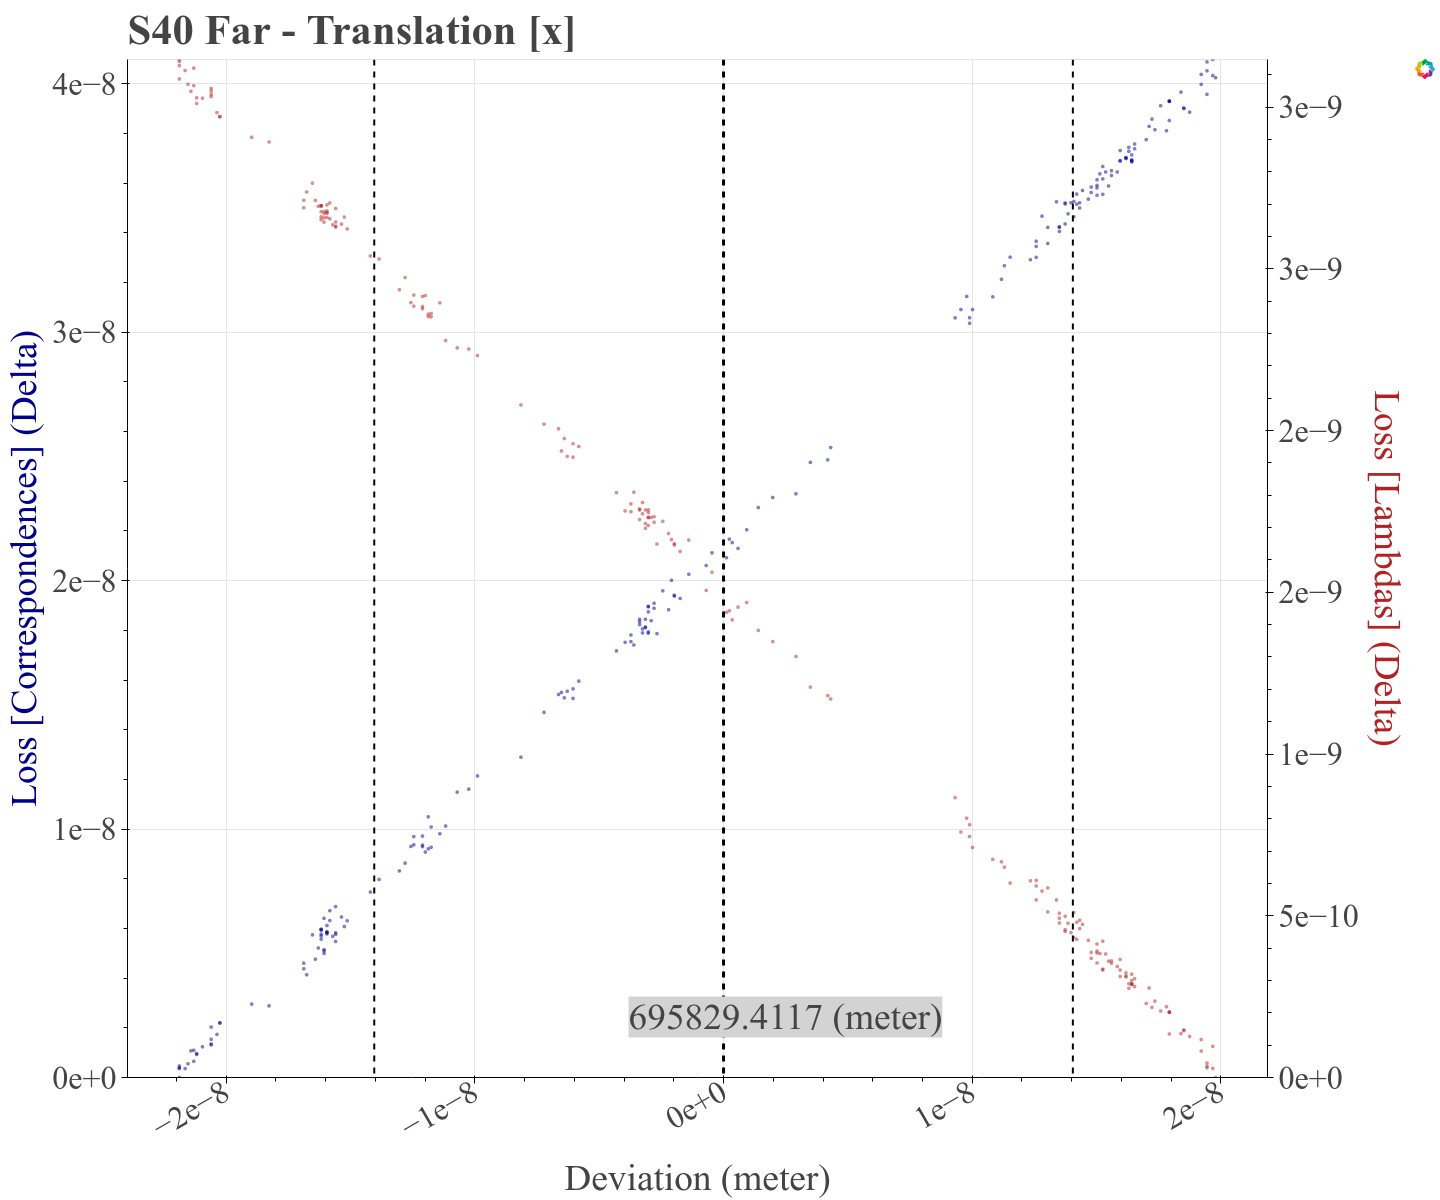
\includegraphics[width=0.45 \linewidth]{diagrams/calibration/s40_n_far/parameters.csv/Translation[x]_vs_Loss[Correspondences]_vs_Loss[Lambdas]_cluster_All.png} &
    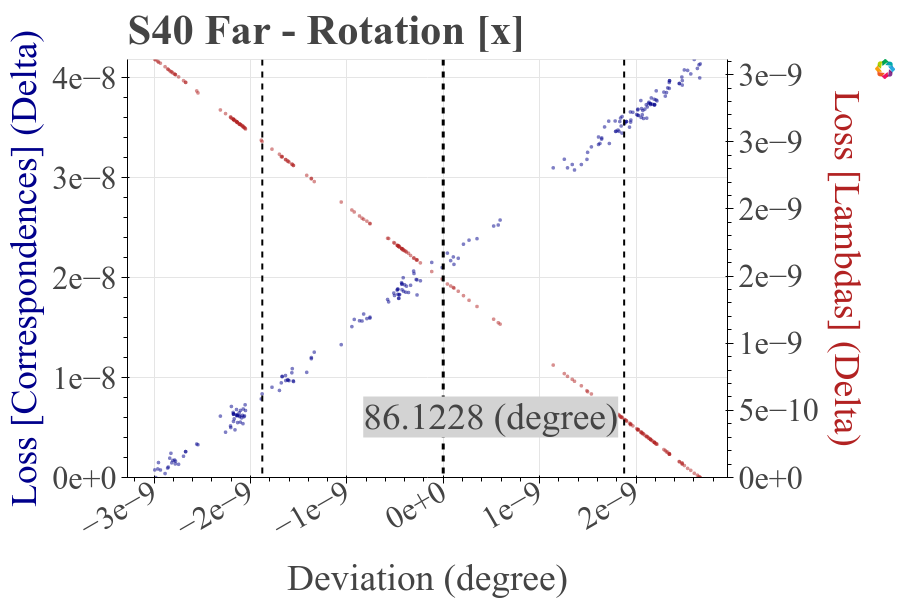
\includegraphics[width=0.45 \linewidth]{diagrams/calibration/s40_n_far/parameters.csv/Rotation[x]_vs_Loss[Correspondences]_vs_Loss[Lambdas]_cluster_All.png} \\
    
    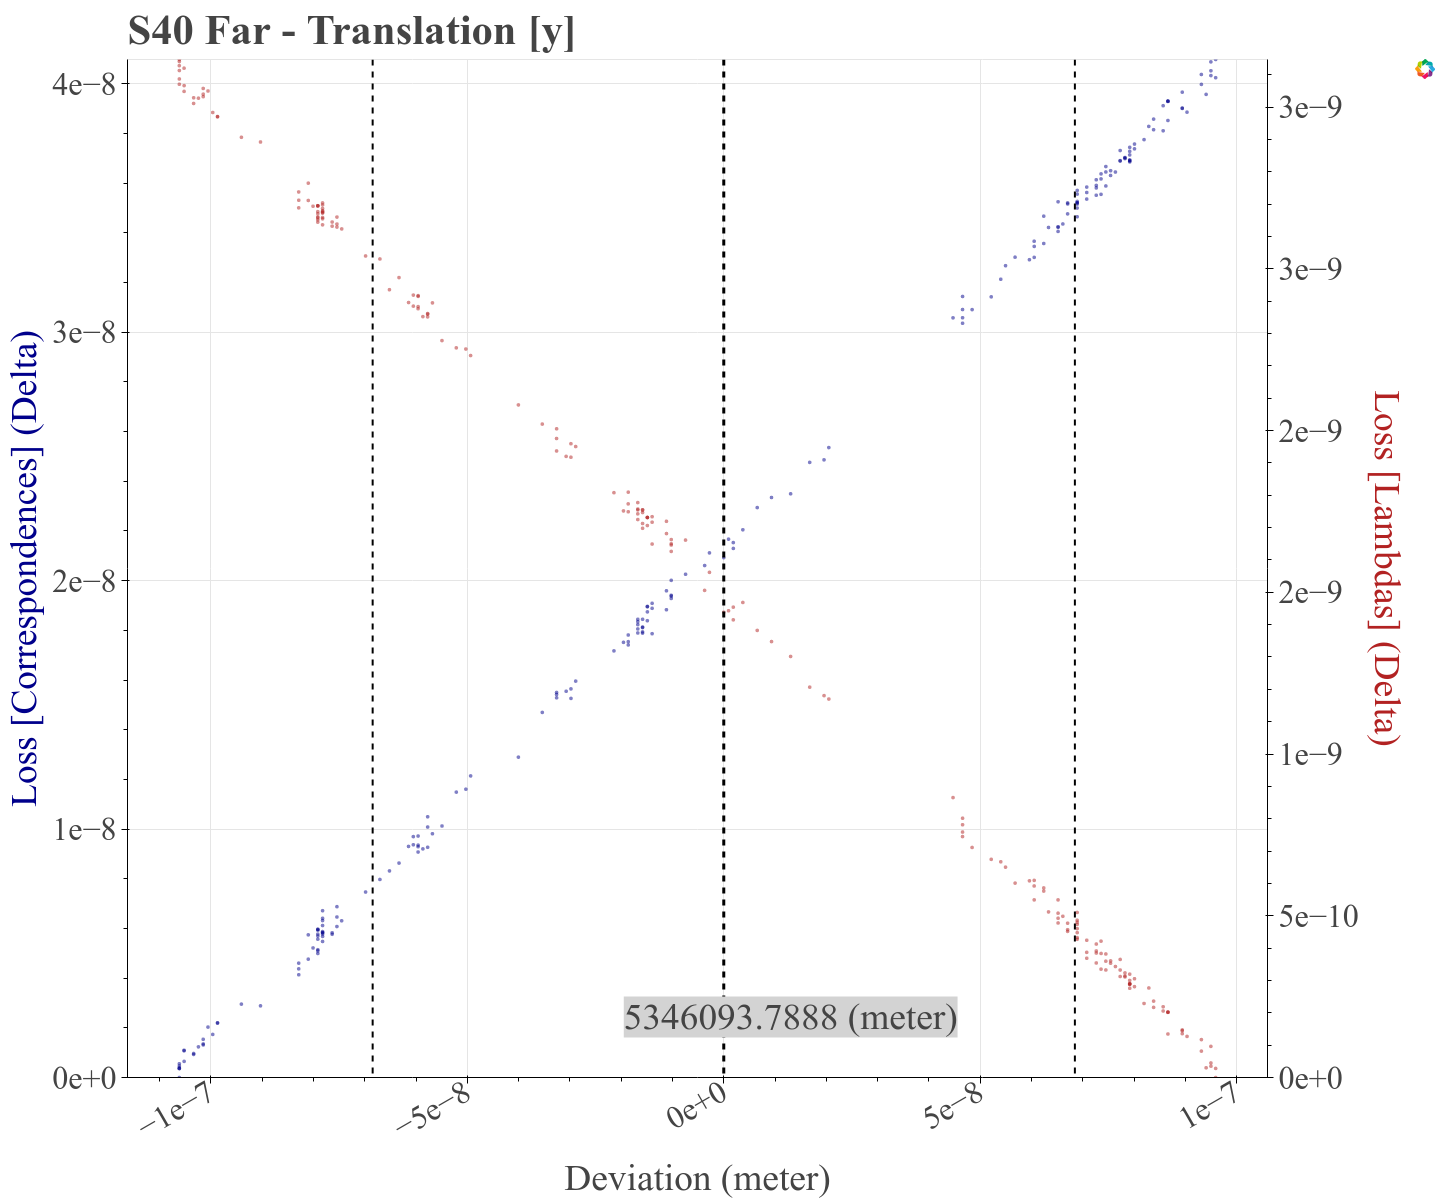
\includegraphics[width=0.45 \linewidth]{diagrams/calibration/s40_n_far/parameters.csv/Translation[y]_vs_Loss[Correspondences]_vs_Loss[Lambdas]_cluster_All.png} &
    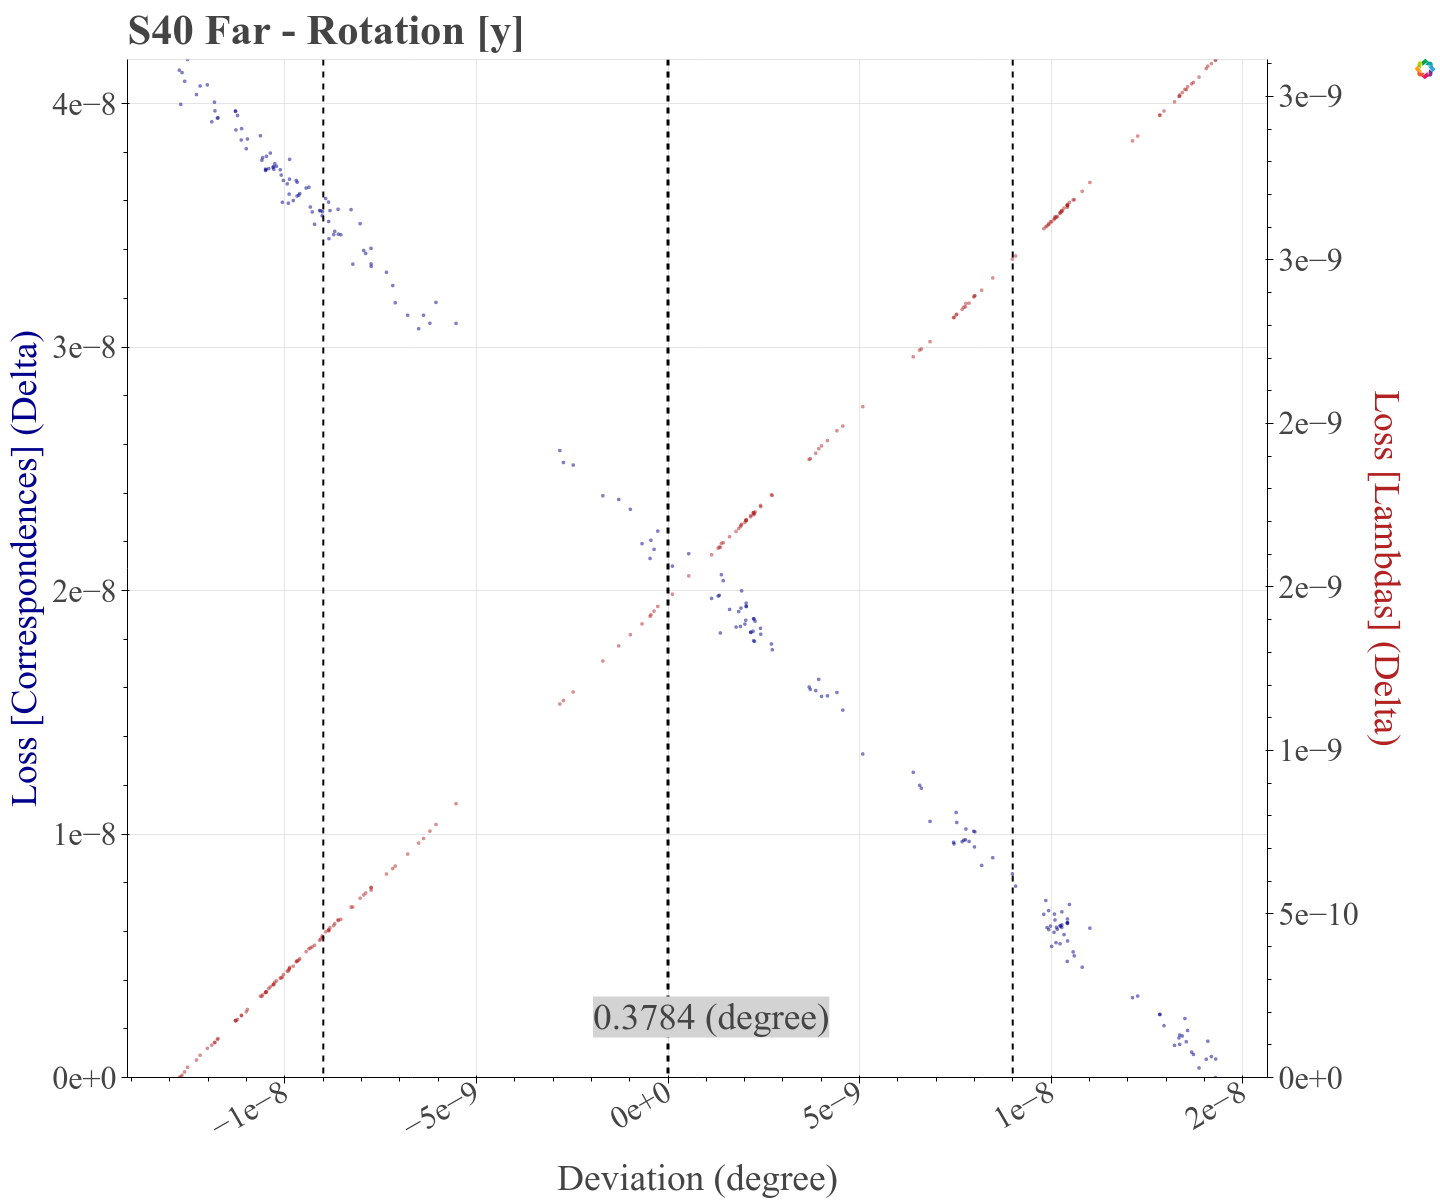
\includegraphics[width=0.45 \linewidth]{diagrams/calibration/s40_n_far/parameters.csv/Rotation[y]_vs_Loss[Correspondences]_vs_Loss[Lambdas]_cluster_All.png} \\
    
    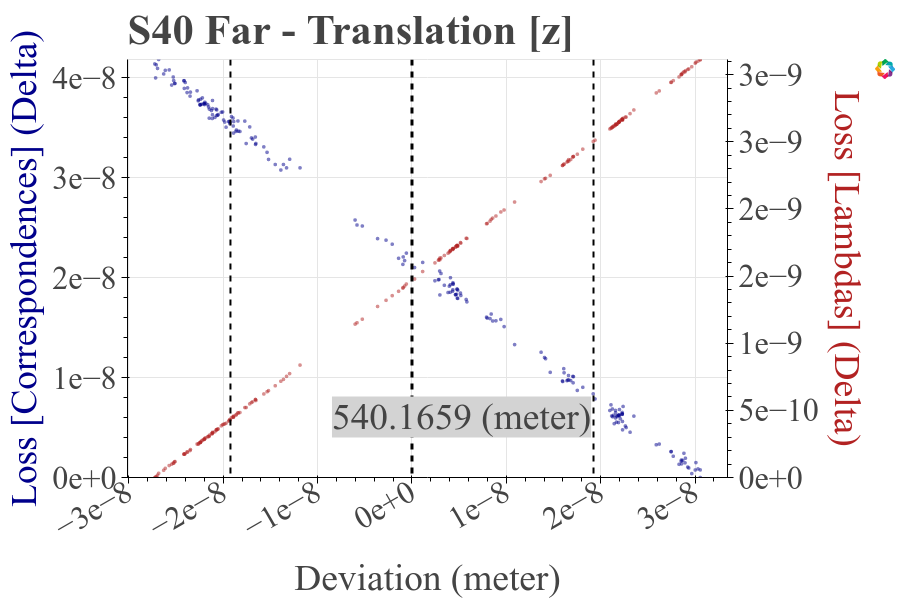
\includegraphics[width=0.45 \linewidth]{diagrams/calibration/s40_n_far/parameters.csv/Translation[z]_vs_Loss[Correspondences]_vs_Loss[Lambdas]_cluster_All.png} &
    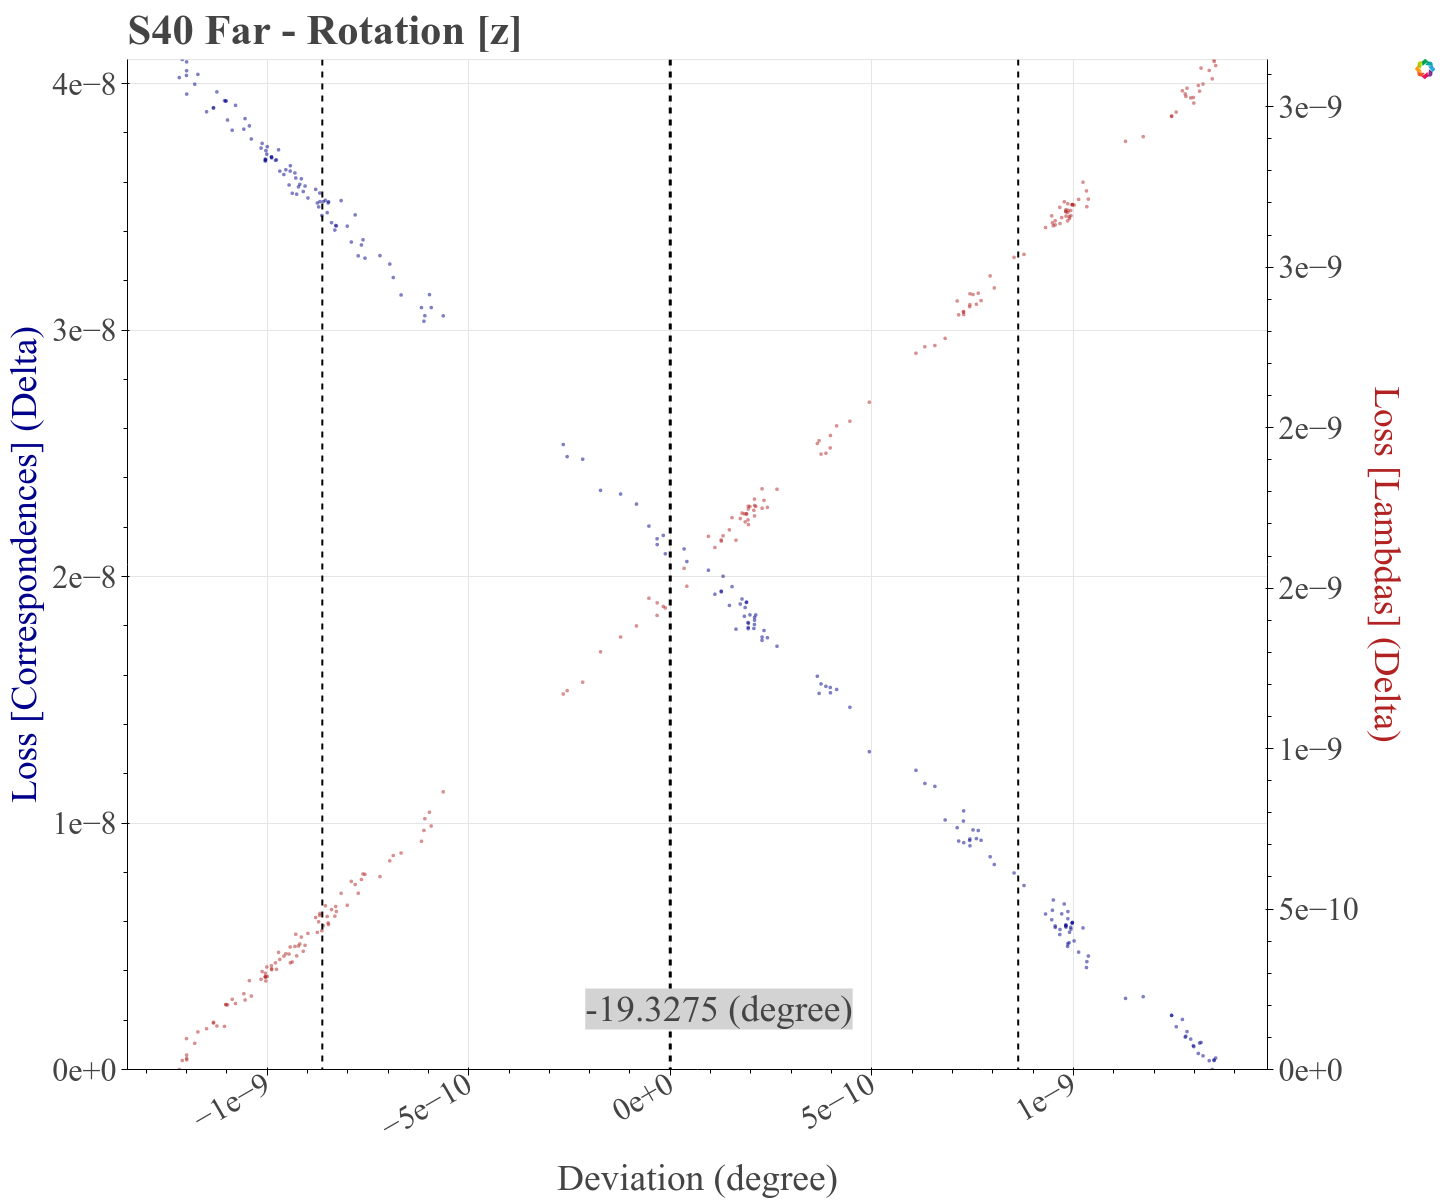
\includegraphics[width=0.45 \linewidth]{diagrams/calibration/s40_n_far/parameters.csv/Rotation[z]_vs_Loss[Correspondences]_vs_Loss[Lambdas]_cluster_All.png} \\

    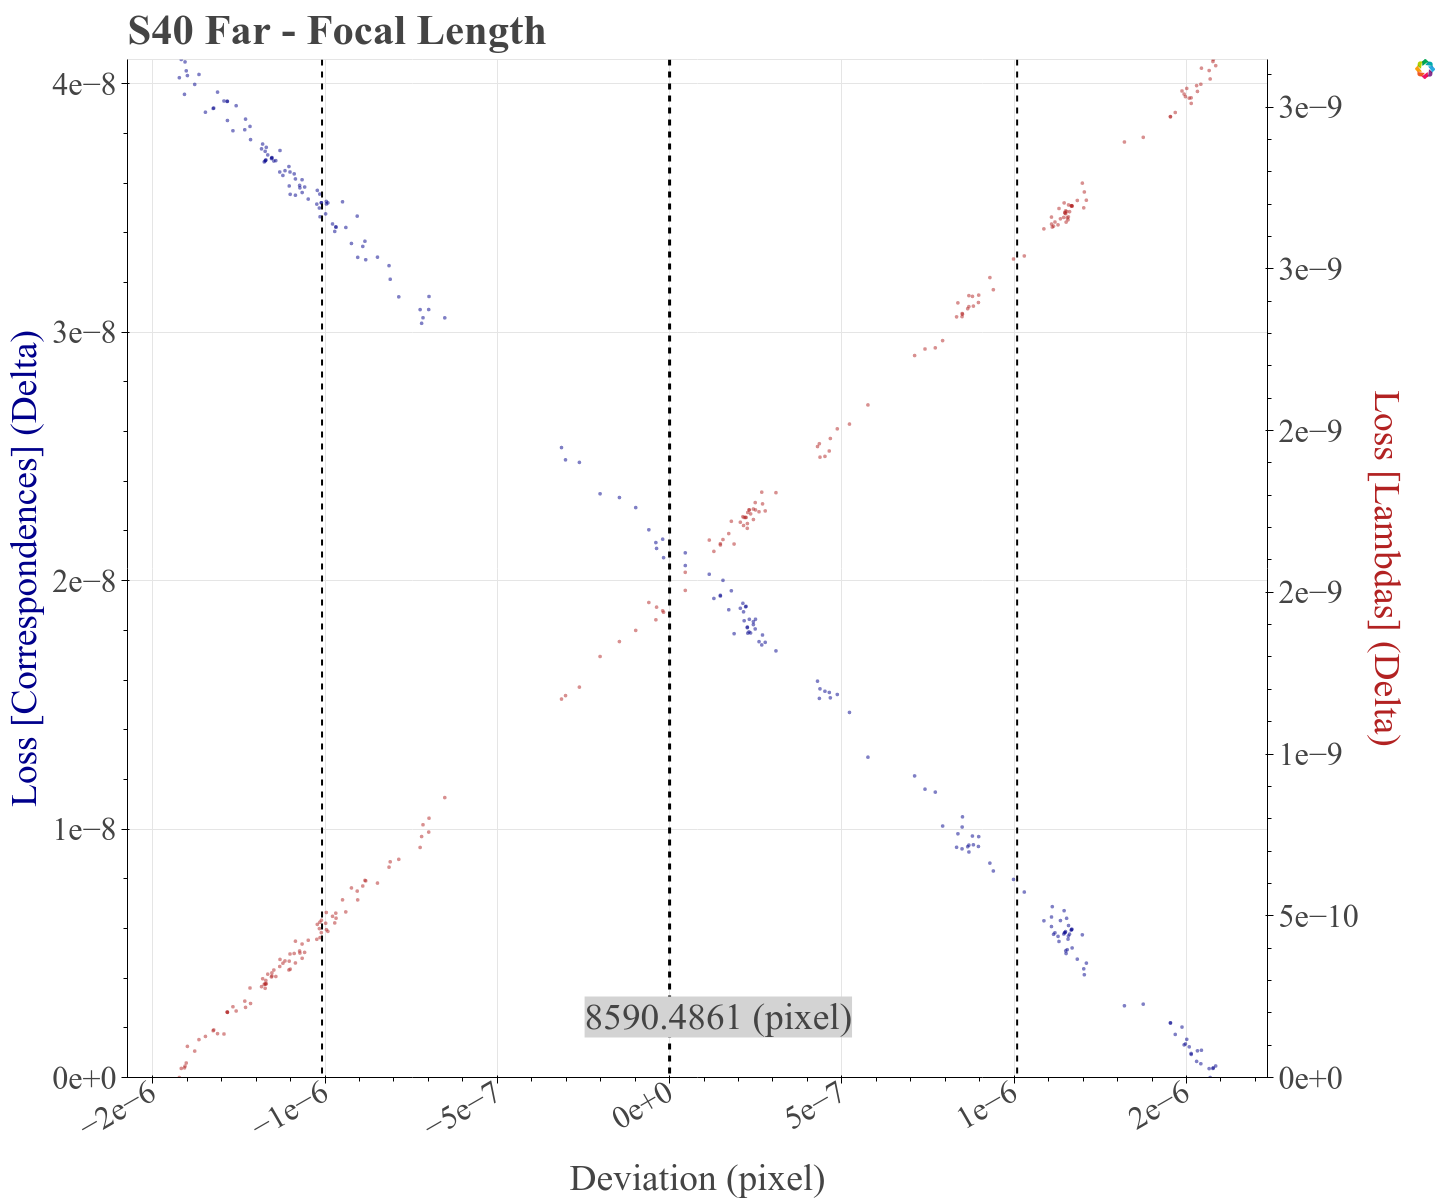
\includegraphics[width=0.45 \linewidth]{diagrams/calibration/s40_n_far/parameters.csv/FocalLength_vs_Loss[Correspondences]_vs_Loss[Lambdas]_cluster_All.png} \\
\end{tabular}
\caption{
  Left: The resulting translational parameters plotted against the remaining losses. 
  Right: The resulting rotational parameters plotted against the remaining losses.
  Bottom: The resulting focal length  plotted against the remaining losses.
  }
\label{fig:static_calibration_algorithmic_error}
\end{figure}

\autoref{fig:static_calibration_algorithmic_error} displays the resulting parameters for the camera \camsf{4}.
We plot each of the parameters against the scale of the remaining loss of the correspondences and the $\lambda_c$.
The translation parameters are in meters and relative to the UTM projection \cite{langley1998utm}.
The rotation parameters are in degrees of Euler angles.

The plots show that the standard deviation $\sigma_T$ of the translations does not exceed $6 * 10^{-8} m = 60 nm$, $\sigma_R$ of the rotation is at most $2 * 10^{-9} deg$ and $\sigma_{\pi}$ of the focal length is at most $1 * 10^{-6}$ pixels.
This implies that compared to the uncertainty introduced by the measurements (\autoref{sec:static_calibration_expectable_error}) the algorithmic error can be neglected.   

We evaluate the algorithmic error for the remaining cameras in the Appendix (\autoref{sec:appendix}). 
The results are the same as expected.

% \subsubsection{Minimal number of correspondences}
